\section*{Energy Calibration}

Before proceeding to study the branching ratio each detector have to be energy calibrated. In order to do so, a $^{22}$Na source was used due to the fact that, NaI(Tl) scintillators, are sensible to photopeak so is possible to use the 511 and  1275 keV photopeak of the sodium source for the purpose of rescaling energy spectra. Calibrated spectrum for each detector is presented in Fig.~\ref{Fig: calibrated spectra}.

\begin{figure}[H]
\centering
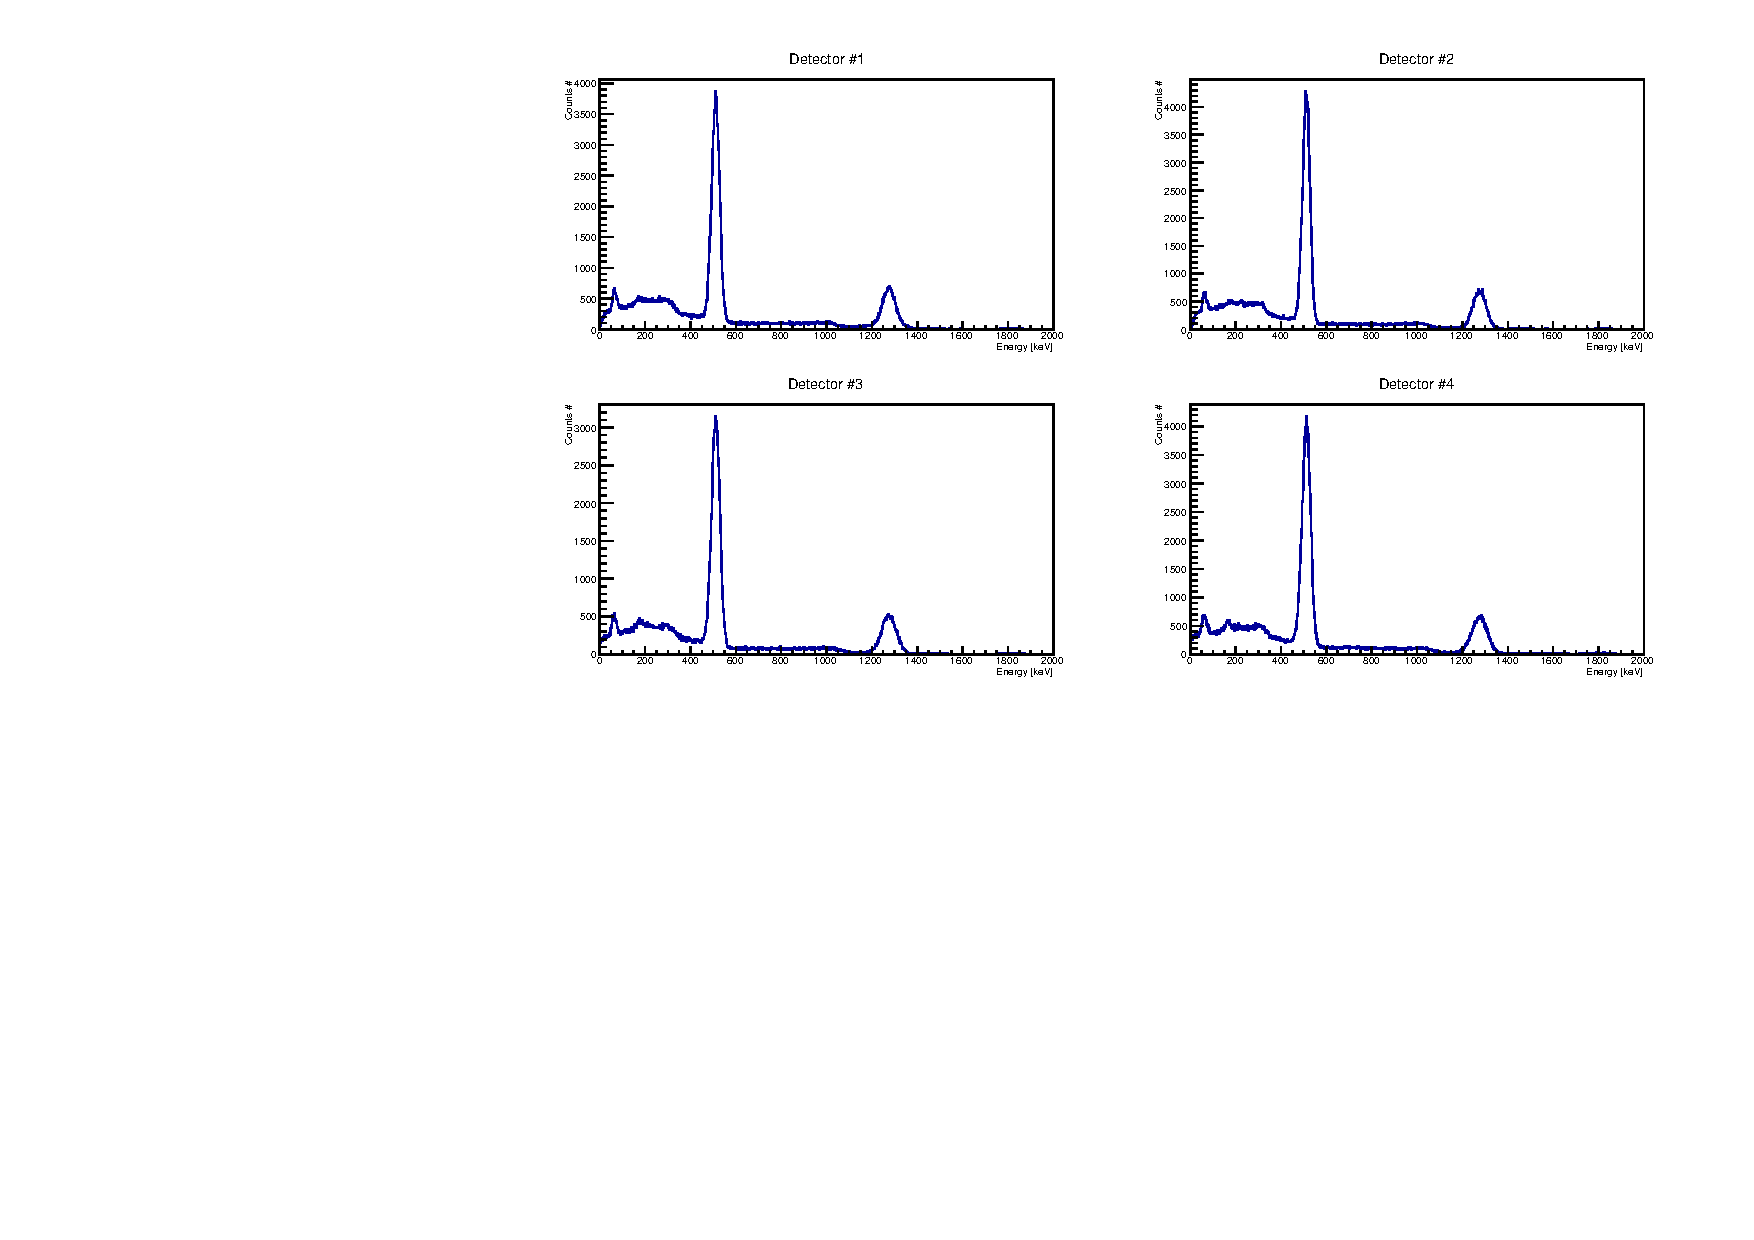
\includegraphics[width = \textwidth]{calibrated_spectra}
\caption{Calibrated $^{22}$Na energy spectra.}
\label{Fig: calibrated spectra}
\end{figure}

% Capire che errore piazzare sui parametri dei fit

\section*{TAC Calibration}

